\section*{Proof by picture: A selection of nice picture proofs}
\vspace{-.30cm}
\label{Britz}


\title{Proof by picture: A selection of nice picture proofs}


\begin{center}
\textbf{Thomas Britz}\footnote{%
Thomas Britz is a Lecturer in the School of Mathematics and Statistics, UNSW, Australia ({\tt britz@unsw.edu.au})},
\textbf{Adam Mammoliti}\footnote{%
Adam Mammoliti is a PhD student in the School of Mathematics and Statistics, UNSW, Australia ({\tt a.mammoliti@unsw.edu.au})}
\textbf{and Henrik Kragh S{\o}rensen}\footnote{%
Henrik S{\o}rensen is a Professor in the Centre for Science Studies, Aarhus University ({\tt hks@ivs.au.dk})}
\end{center}

\vspace{5mm}
%\section{Introduction and statement of aim}

Just like any other cultural group, mathematicians like to tell stories.
We tell heroic stories about famous mathematicians,
%to display our lineage and
to inspire or reinforce our cultural values,
and we encase our results in narratives to explain how they
are interesting and how they relate to other results.
%%
We also tell stories to convince others that our results are valid,
and preferably also to explain why they are true.
These stories are what you know as ``proofs".

You might think (perhaps with some trepidation) of proofs as formal,
written sequences of logical steps.
However, proofs can come in a variety of formats,
some of which are more active or intuitive than a formal written proof.
In this article, we show how proofs can be in the form of pictures,
and we show a selection of these picture proofs
that we find particularly elegant and instructive.

\medskip

\subsection*{A classic way to add integers}
\noindent
Let us begin with one of our favourite picture proofs,
of the following identity (which is not quite as interesting as its various proofs).
\begin{theorem}
\label{thm:integer_sum}
\[
  1 + 2 + \cdots + n = \frac{1}{2}n(n+1)
\]
\end{theorem}
%Here, $n$ is some positive integer.

\noindent {\em Proof}

\newcommand{\mycircle}[2]{\fill[fill=white!75!gray,draw=black] (#1,#2) circle (3mm);}

\newcommand\xc{1.73}
\newcommand\zc{1}
\newcommand\nn{3} % This parameter is only 100% useful for \pyramida - but does work nicely for that case

\begin{center}
  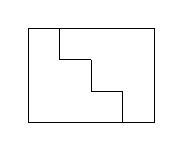
\begin{tikzpicture}[scale=.2]
    \begin{scope}[shift={(0,0)}]
      \fill[fill=white!100!gray,draw=black] (0,0) rectangle (2*\nn + 2, 2*\nn);
      \foreach \x in {1,...,\nn}{
        \draw (2*\x,2*\nn+2-2*\x) -- ++(0,-2) -- ++(2,0);}
    \end{scope}
  \end{tikzpicture}
\end{center}

Each of the two regions demarked in the rectangle above
consists of $1 + 2 + \cdots + n$ squares (here, $n = 3$).
The rectangle has $n$ rows of squares and $n+1$ columns,
so the rectangle consists of $n(n+1)$ squares in total.
Each of the two regions is half of this number,
just as the theorem states.  \hfill$\square$

\medskip

\subsection*{A different way to add integers}
\noindent
Looking at the term $\frac{1}{2}n(n+1)$ gives us a clue for another picture proof
of Theorem~\ref{thm:integer_sum}.
This term, also written as the {\em binomial coefficient} $\binom{n+1}{2}$,
is the number of ways of choosing two things out of an unordered collection of $n+1$ things.
For instance, if we have $n + 1 = 10$ people and want to count the ways in which any two of them
can shake hands, then we could first choose any one of the people (10 choices)
and then choose a second person from the remaining nine people (9 choices).
This will give $10\times 9 = 90$ choices, but we have counted the handshakes twice.
For instance, choosing Ada and then Ben, and later choosing Ben and then Ada.
The number of handshakes is therefore $\frac{1}{2}\times 90 = 45$, or $\binom{n+1}{2} = \frac{1}{2}n(n+1)$.
The following picture proof expresses the sum $1 + 2 + \cdots + n$ as
the white circles in the first $n$ rows, where $n=3$ here.

\begin{center}
  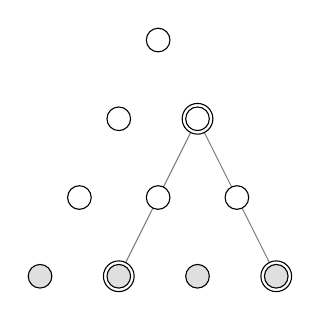
\begin{tikzpicture}[scale=.5]
    \begin{scope}[shift={(0,0)}]
    \draw[gray] (\nn-3,-2*\nn-2) -- (\nn-1,-2*\nn+2) -- (\nn+1,-2*\nn-2);
    \fill[fill=white,draw=black] (\nn-3,-2*\nn-2) circle (3.9mm);
    \fill[fill=white,draw=black] (\nn+1,-2*\nn-2) circle (3.9mm);
    \fill[fill=white,draw=black] (\nn-1,-2*\nn+2) circle (3.9mm);
      \foreach \y in {1,...,\nn}{
        \foreach \x in {1,...,\y}{
          \fill[fill=white,draw=black] (-\y+2*\x,-2*\y) circle (3mm);}}
      \foreach \x in {1,...,\nn}{
        \fill[fill=white!75!gray,draw=black] (-\nn-\zc+2*\x,-2*\nn-2) circle (3mm);}
      \fill[fill=white!75!gray,draw=black] (\nn+1,-2*\nn-2) circle (3mm);
    \end{scope}
%    \fill[fill=white!50!gray,draw=black] (\nn-3,-2*\nn-2) circle (3mm);
%    \fill[fill=white!50!gray,draw=black] (\nn+1,-2*\nn-2) circle (3mm);
%    \fill[fill=white!50!gray,draw=black] (\nn-1,-2*\nn+2) circle (3mm);
%    \mycircle{\nn-1,-2*\nn+2}
  \end{tikzpicture}
\end{center}

The bottom row has $n+1$ grey circles,
and any choice of two of these corresponds to exactly one of the white circles,
and vice versa; this is illustrated by the three encircled circles.
So, instead of counting white circles,
we can count the ways of choosing any 2 of the grey circles, and this number is, as we have seen,
$\binom{n+1}{2} = \frac{1}{2}n(n+1)$.\footnote{This elegant proof was first presented,
along with many other proofs,
in [L.C.~Larson, {\sl A discrete look at $1+2+\cdots+n$},
College Math.\ Journal~{\bf 16} (1985), 369--382].}

\medskip

\subsection*{How to add squares, or how to play with LEGO}
\noindent
We have seen how to count the sum $1 + 2 + \cdots + n$ by drawing pictures.
What about the sum of squares?
It turns out that this is also not so hard:

\begin{theorem}
\label{thm:square_sum}
\[
  1^2 + 2^2 + \cdots + n^2 = \frac{1}{6}n(n+1)(2n+1)
\]
\end{theorem}

By looking at the term $\frac{1}{6}n(n+1)(2n+1)$
and by thinking about our simpler sum,
we might be inspired to form a rectangle-type object with side lengths $n$, $n+1$, and $2n+1$
out of 6 triangle-type objects, which, given that we are now working in three dimensions,
would probably be pyramid-type objects.
This does in fact give us our proof:%
\footnote{Thomas discovered this proof when he was still a student,
  during a particularly boring lecture.
  It had already been discovered, however, presumably many times,
  the first known instance being by Yang Hui in 1261 AD
  (see [M.-K.~Sui, {\sl Pyramid, pile, and sum of squares},
   Historia Math.~{\bf 8} (1981), 61--66]).}

\newcommand{\pyramid}[1]{
  \foreach \x in {1,...,#1}{
    \fill[fill=white!50!gray,draw=black] (\x*2*\xc,0) -- ++(\xc,-\zc) -- ++(0,#1*2*\zc+2*\zc-\x*2*\zc) -- ++(-\xc,\zc) -- cycle;
    \fill[fill=white        ,draw=black] (\x*2*\xc,#1*2*\zc+2*\zc -\x*2*\zc) -- ++(\xc,-\zc) -- ++(#1*\xc+\xc-\x*\xc,#1*\zc+\zc-\x*\zc) -- ++(-\xc,\zc) -- cycle;
    \fill[fill=white!75!gray,draw=black] (\x*2*\xc+\xc,-\zc) -- ++(0,#1*2*\zc+2*\zc -\x*2*\zc) -- ++(#1*\xc+\xc-\x*\xc,#1*\zc+\zc-\x*\zc) -- ++(0,-#1*2*\zc-2*\zc +\x*2*\zc) -- cycle;}}

\newcommand{\pyramida}{\pyramid{\nn}}

\newcommand{\pyramidb}{
  \fill[  fill=white        ,draw=black] (0,2*\zc) -- ++(0,\nn*2*\zc-2*\zc) -- ++(\xc,\zc) -- ++(\nn*2*\xc-\xc,-\nn*2*\zc+\zc) -- ++(-\nn*\xc,-\nn*\zc) -- cycle;
  \foreach \x in {1,...,\nn}{
    \fill[fill=white!75!gray,draw=black] (\x*\xc,\nn*2*\zc+2*\zc-\x*3*\zc) -- ++(0,-2*\zc) -- ++(\x*\xc,\x*\zc) -- ++(0,2*\zc) -- cycle;}
  \fill[  fill=white!50!gray,draw=black] (0,0) -- ++(0,\nn*2*\zc) -- ++(\xc,-\zc) -- ++(0,-2*\zc) -- ++(\xc,-\zc) -- ++(0,-2*\zc) -- ++(\xc,-\zc) -- ++(0,-2*\zc) -- cycle;}

\newcommand{\pyramidc}{
  \fill[  fill=white!50!gray,draw=black] (0,0) -- ++(0,2*\zc) -- ++(\nn*2*\xc-2*\xc,0) -- ++(\xc,-\zc) -- ++(0,-\nn*2*\zc) -- cycle;
  \fill[  fill=white        ,draw=black] (0,2*\zc) -- ++(\xc,-\zc) -- ++(\xc,\zc) -- ++(\xc,-\zc) -- ++(\xc,\zc) -- ++(\xc,-\zc) -- ++(\xc,\zc) -- ++(-\nn*\xc,\nn*\zc) -- cycle;
  \foreach \x in {1,...,\nn}{
    \fill[fill=white!75!gray,draw=black] (\x*2*\xc-\xc,\zc) -- ++(\xc,\zc) -- ++(0,-\x*2*\zc) -- ++(-\xc,-\zc) -- cycle;}}

\newcommand{\pyramidabc}{
  \pyramida
  \fill[  fill=white        ,draw=black] (\nn*\xc+3*\xc,\nn*3*\zc+\zc) -- ++(\xc,-\zc) -- ++(\xc,\zc) -- ++(\xc,-\zc) -- ++(\xc,\zc) -- ++(\xc,-\zc) -- ++(\xc,\zc) -- ++(-\nn*\xc,\nn*\zc) -- cycle;
  \foreach \x in {1,...,\nn}{
    \fill[fill=white        ,draw=black] (\nn*\xc+  \xc+\x*\xc,\nn*3*\zc+3*\zc-\x*3*\zc) -- ++(\xc,-\zc) -- ++(\x*\xc,\x*\zc) -- ++(-\xc,\zc) -- cycle;
    \fill[fill=white!75!gray,draw=black] (\nn*\xc+2*\xc+\x*\xc,\nn*3*\zc+2*\zc-\x*3*\zc) -- ++(0,-2*\zc) -- ++(\x*\xc,\x*\zc) -- ++(0,2*\zc) -- cycle;
    \fill[fill=white!75!gray,draw=black] (\nn*\xc+2*\xc+\x*2*\xc,\nn*3*\zc) -- ++(\xc,\zc) -- ++(0,-\x*2*\zc) -- ++(-\xc,-\zc) -- cycle;}
  \foreach \x in {1,2}
    \fill[fill=white!50!gray,draw=black] (\nn*\xc+3*\xc+\x*2*\xc,\nn*3*\zc+\zc) -- ++(\xc,-\zc) -- ++(0,-\x*2*\zc) -- ++(-\xc,\zc) -- cycle;}

\newcommand{\pyramide}{
  \foreach \r in {0,50}{
    \fill[fill=gray!\r!white,draw=black,rotate=-\r*120/25] (0,0) -- ++(-\nn*\xc,\nn*\zc) -- ++(\xc,\zc) --
      ++(\xc,-\zc) -- ++(\xc,\zc) -- ++(\xc,-\zc) -- ++(\xc,\zc) -- ++(\xc,-\zc) -- cycle;}
    \fill[fill=gray!25!white,draw=black] (0,0) -- ++(0,-\nn*2*\zc) -- ++(\nn*\xc,\nn*\zc) -- ++(0,\nn*2*\zc) -- cycle;}

\newcommand{\pyramidf}{
  \fill[fill=white          ,draw=black] (0,0) -- ++(-\nn*\xc, \nn*\zc) -- ++(\nn*\xc,\nn*\zc) -- ++(\nn*\xc,-\nn*\zc) -- cycle;
  \fill[fill=white!50!gray  ,draw=black] (-\nn*\xc,\nn*\zc) -- ++(0,-2*\zc) -- ++(\nn*\xc+2*\xc,-\nn*\zc-2*\zc) -- ++(0,2*\zc) -- cycle;
  \fill[fill=white!75!gray  ,draw=black] (0,0) -- ++(0,-2*\zc) -- ++(\xc,\zc) -- ++(0,-2*\zc) -- ++(\xc,\zc) -- ++(0,-2*\zc) -- ++(\xc,\zc) -- ++(0,\nn*2*\zc) -- cycle;}

\newcommand{\pyramidg}{
  \fill[fill=white          ,draw=black] (-\nn*\xc,\nn*\zc) -- ++(\xc,\zc) -- ++(\nn*\xc+2*\xc,-\nn*\zc-2*\zc) -- ++(-\xc,-\zc) -- cycle;
  \fill[fill=white!50!gray  ,draw=black] (0,0) -- ++(0,-\nn*2*\zc) -- ++(-\nn*\xc,\nn*\zc) -- ++(0,\nn*2*\zc) -- cycle;
  \fill[fill=white!75!gray  ,draw=black] (0,0) -- ++(\xc,\zc) -- ++(0,-2*\zc) -- ++(\xc,\zc) -- ++(0,-2*\zc) -- ++(\xc,\zc) -- ++(0,-2*\zc) -- ++(-\nn*\xc,-\nn*\zc) -- cycle;}

\newcommand{\pyramidefg}{
  \fill[fill=white          ,draw=black] (0,0) -- ++(-\nn*\xc,\nn*\zc) -- ++(\nn*\xc+2*\xc,\nn*\zc+2*\zc) -- ++(\xc,-\zc) -- ++(\xc,\zc) -- ++(\xc,-\zc) -- ++(\xc,\zc) -- ++(\xc,-\zc) -- cycle;
  \fill[fill=white!50!gray  ,draw=black] (0,0) -- ++(0,-\nn*2*\zc) -- ++(-\nn*\xc,\nn*\zc) -- ++(0,\nn*2*\zc) -- cycle;
  \fill[fill=white!75!gray  ,draw=black] (0,0) -- ++(0,-\nn*2*\zc) -- ++(\nn*2*\xc+\xc,\nn*2*\zc+\zc) -- ++(0,\nn*2*\zc) -- cycle;
  \draw (\xc,\zc) -- ++(0,-2*\zc) -- ++(\xc,\zc) -- ++(0,-2*\zc) -- ++(\xc,\zc) -- ++(0,-2*\zc);
  \draw (\xc,\zc) -- ++(-\nn*\xc,\nn*\zc);
  \draw (\nn*\xc+\xc,-\nn*\zc+\zc) -- ++(0,\nn*2*\zc) -- ++(-\nn*\xc,\nn*\zc);}

\newcommand{\brick}{
  \fill[fill=white          ,draw=black] (0,0) -- ++(-\nn*\xc-\xc,\nn*\zc+\zc) -- ++(\nn*2*\xc+\xc,\nn*2*\zc+\zc) -- ++(\nn*\xc+\xc,-\nn*\zc-\zc) -- cycle;
  \fill[fill=white!50!gray  ,draw=black] (0,0) -- ++(0,-\nn*2*\zc) -- ++(-\nn*\xc-\xc,\nn*\zc+\zc) -- ++(0,\nn*2*\zc) -- cycle;
  \fill[fill=white!75!gray  ,draw=black] (0,0) -- ++(0,-\nn*2*\zc) -- ++(\nn*2*\xc+\xc,\nn*2*\zc+\zc) -- ++(0,\nn*2*\zc) -- cycle;
  \draw (-\nn*\xc+\xc, \nn*\zc+\zc) -- ++(\nn*\xc,-\nn*\zc) -- ++(0,-2*\zc) -- ++(\xc,\zc) -- ++(0,-2*\zc) -- ++(\xc,\zc) -- ++(0,-2*\zc);
  \draw ( \nn*\xc+\xc,-\nn*\zc+\zc) -- ++(0,\nn*2*\zc) -- ++(-\nn*\xc-\xc,\nn*\zc+\zc);
  \draw (-\nn*\xc    ,-\nn*\zc    ) -- ++(0,\nn*2*\zc) -- ++(\nn*\xc+2*\xc,\nn*\zc+2*\zc) -- ++(\xc,-\zc) -- ++(\xc,\zc) -- ++(\xc,-\zc) -- ++(\xc,\zc);}

\begin{center}
  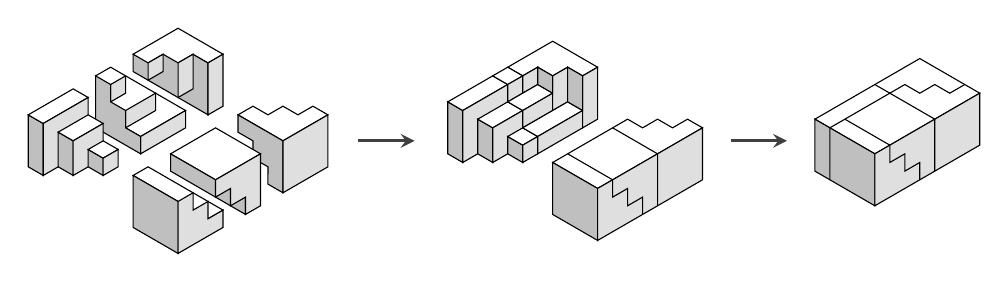
\begin{tikzpicture}[scale=.11,shift={(2,0)}]
    \begin{scope}[shift={(        0,        0)}]  \pyramidc   \end{scope}
    \begin{scope}[shift={( -2.5*\xc, -6.5*\zc)}]  \pyramidb   \end{scope}
    \begin{scope}[shift={(   -9*\xc,-11  *\zc)}]  \pyramida   \end{scope}
    \begin{scope}[shift={( 10  *\xc, -8  *\zc)}]  \pyramide   \end{scope}
    \begin{scope}[shift={(  5.5*\xc,-12.5*\zc)}]  \pyramidf   \end{scope}
    \begin{scope}[shift={(  3  *\xc,-15  *\zc)}]  \pyramidg   \end{scope}
    \draw[draw=darkgray, very thick,>=stealth,->] (26,-8) -- (32.5,-8);
    \begin{scope}[shift={( 19  *\xc, -9.5*\zc)}]  \pyramidabc \end{scope}
    \begin{scope}[shift={( 31  *\xc,-13.5*\zc)}]  \pyramidefg \end{scope}
    \draw[draw=darkgray, very thick,>=stealth,->] (69,-8) -- (75.5,-8);
    \begin{scope}[shift={( 49.5*\xc, -9.5*\zc)}]  \brick \end{scope}
  \end{tikzpicture}
\end{center}

It could be a little hard to visualise how the middle of the rectangle fits together,
so we made a YouTube video in which we built the pyramids in LEGO and put them together.
You can find the video here:

\centerline{\url{https://www.youtube.com/watch?v=p8dL7kHMsII}}

(Alternatively, you can google ``LEGO proof YouTube".)

\medskip

%\section{Arguing with and about graphs}

\subsection*{Love/hate-triangles among six people}
\noindent
So far, our proofs have used pictures to prove algebraic identities.
We will now use pictures to prove a mathematical result
that could itself be seen as a picture.

Imagine putting six people in a room together and letting them get to know each other.
One person might like or dislike some of the others,
or not really care about them, say.
Suppose, though, that each pair of these people either forms a mutual like or
mutual dislike to each other.
We can draw this situation by drawing a {\em graph} in which
each person is represented by a circle,
and any two people are connected by a line
that is either white (\begin{tikzpicture}[scale=1]
   \coordinate (A) at (0,0);
   \coordinate (B) at (.5,0);
   \draw[white] (0,-.12) -- (A);
   \draw[gray ,very thick] (B) -- (A);
   \draw[white,     thick] (B) -- (A);\end{tikzpicture})
if they like each other
or black (\begin{tikzpicture}[scale=1]
   \draw[white] (0,-.12) -- (0,0);
   \draw[black,very thick] (0,0) -- (.5,0);\end{tikzpicture}) if they don't:

\begin{center}
  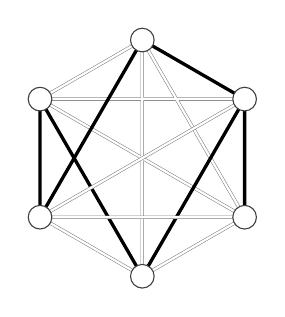
\begin{tikzpicture}[scale=.5]
    % I first tried to define coordinates and make loops of them but couldn't quickly see how to do this
%      \foreach \xb/\yb in {2.598/1.5,2.598/-1.5,-2.598/1.5,-2.598/-1.5,0/3,0/-3}{
 %       \draw[green!value(round(rand))!red] (\xa,\ya)--(\xb,\yb);};
    \foreach \rr/\na in {1/A,2/B,3/C,4/D,5/E,6/F}{\coordinate (\na) at (30+60*\rr:3);};
    \draw[gray ,very thick] (A) -- (B) (A) -- (E) (B) -- (E) (B) -- (F) (A) -- (D);
    \draw[white,     thick] (A) -- (B) (A) -- (E) (B) -- (E) (B) -- (F) (A) -- (D);
    \draw[black,very thick] (A) -- (C) (B) -- (D) (A) -- (F) (B) -- (C) (D) -- (F) (E) -- (F);
    \draw[gray ,very thick] (C) -- (D) (C) -- (E) (C) -- (F) (D) -- (E);
    \draw[white,     thick] (C) -- (D) (C) -- (E) (C) -- (F) (D) -- (E);
    \foreach \na in {A,...,F}{
      \fill[fill=white!100!gray,draw=darkgray] (\na) circle (3mm);};
  \end{tikzpicture}
\end{center}

\begin{theorem}
\label{thm:R33}
Among any six people as described above,
you can always find three people who pairwise like each other
or three people who pairwise dislike each other.
\end{theorem}

In pictures, the theorem states that
there will always be either a white triangle or a black triangle.
In the specific example above,
there are no black triangles but there are  white triangles.
This is a simple case of {\em Ramsey Theory} which is a beautiful but difficult mathematical area.

\medskip

\noindent {\em Proof}

Look at one particular person and consider the 5 lines that connect that person.
Of~those lines, at least 3 must be white or at least 3 must be black.
Let us suppose that at least 3 are white,
perhaps as in Case~1 below:

\newcommand{\casesa}[4]{\begin{scope}[shift={(#1,#2)}]
    \foreach \rr/\na in {1/A,2/B,3/C,4/D,5/E,6/F}{\coordinate (\na) at (30+60*\rr:3);};
    \draw[gray ,very thick] (A) -- (C) (A) -- (D) (A) -- (E); #3
    \draw[white,     thick] (A) -- (C) (A) -- (D) (A) -- (E); #3
    \foreach \na in {A,C,D,E}{\fill[fill=white!100!gray,draw=darkgray] (\na) circle (3mm);};
    \node at (0,-4.5) {#4};
  \end{scope}}

\begin{center}
  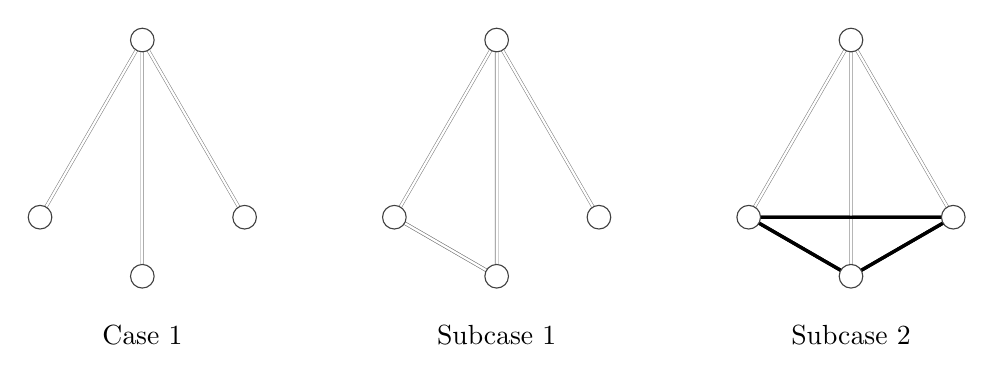
\begin{tikzpicture}[scale=.5,shift={(0,3)}]
    \casesa{ 0}{0}{}{Case 1}
    \casesa{ 9}{0}{\draw[gray ,very thick] (C) -- (D);
                   \draw[white,     thick] (C) -- (D);}{Subcase 1}
    \casesa{18}{0}{\draw[black,very thick] (D) -- (E) (E) -- (C) (C) -- (D);}{Subcase 2}
  \end{tikzpicture}
\end{center}
If, among the 3 people that are thus connected to our first person,
any of two of these like each other (i.e. are connected by a white line),
then we have a white triangle, for instance as in Subcase~1.
%follows:
%\begin{center}
%  \begin{tikzpicture}[scale=.5]
%    \foreach \rr/\na in {1/A,2/B,3/C,4/D,5/E,6/F}{\coordinate (\na) at (30+60*\rr:3);};
%    \draw[green,thick] (A) -- (C) (A) -- (D) (A) -- (E) (C) -- (D) ;
%    \foreach \na in {A,C,D,E}{
%      \fill[fill=white!100!gray,draw=black] (\na) circle (3mm);};
%  \end{tikzpicture}
%\end{center}
However, if no pair of these three people like each other,
then we get a black triangle as in Subcase~2.
%:
%\begin{center}
%  \begin{tikzpicture}[scale=.5]
%    \foreach \rr/\na in {1/A,2/B,3/C,4/D,5/E,6/F}{\coordinate (\na) at (30+60*\rr:3);};
%    \draw[green,thick] (A) -- (C) (A) -- (D) (A) -- (E);
%    \draw[red  ,thick] (D) -- (E) (E) -- (C) (C) -- (D);
%    \foreach \na in {A,C,D,E}{
%      \fill[fill=white!100!gray,draw=black] (\na) circle (3mm);};
%  \end{tikzpicture}
%\end{center}
If the first person had been connected by at least 3 black lines,
then just repeat the above Case~1 considerations with black and white swapped.  \hfill$\square$

\medskip

\subsection*{Figures in elementary geometry}
\noindent
We have now seen pictures used as proofs or as parts of proofs,
as well as pictures being the objects of interest in the theorems themselves.
Moving on to classical Euclidean geometry,
we will now see how pictures can be important for describing the
processes involved in devising and proving theorems.

\medskip

\subsection*{Stating the obvious: Diagrams and geometry}
\noindent
%% Euclid
Euclid's work \textit{The Elements} (c.~295 BC)
is one of the most influential mathematical texts.
Its first book treats elementary planar geometry by deriving theorems from
statements known as ``axioms'' or ``postulates''
that Euclid saw as self-evidently true.
These included statements such as
``when two quantities are each equal to a third quantity,
they are also equal to each other'',
and the postulates that any two points can be joined by a line
and that a circle can be drawn around any centre with any radius.

%% Diagrams in extant sources
%% Constructions and proofs
Euclid's theorems are rigidly presented by a statement of the theorem,
a geometric construction,
and a proof showing that the theorem follows from the construction.
The constructions can be seen as recipes for how to draw diagrams,
and so we see that picture proofs are inherent in Euclid's work.
Some of the oldest still existing sources
--- papyri from c.~300 AD --- display diagrams.

%% Stating the obvious --- and missing axioms
The very first theorem in Euclid's work is encapsuled in the following
diagram and proves the existence of an equilateral triangle on a given line segment.
The construction is to draw the two circles using the segment as their radius and to identify their intersection.
The proof then uses the axioms to prove that the three sides are equal.
The diagram serves both to illustrate the construction and to support the proof.
That is also true for the rest of Euclid's work
which includes much more complicated diagrams.

\begin{center}
  \begin{tikzpicture}[scale=0.4]
    \coordinate (A1) at (1.5,0);
    \coordinate (A2) at ([xscale=-1]A1);
    \node [name path=C1, draw, circle through=(A1)] at (A2) {};
    \node [name path=C2, draw, circle through=(A2)] at (A1) {};
    \path [name intersections={of=C1 and C2, by={A3}}];
    \draw (A1)--(A2)--(A3)--cycle;
    \foreach \n in {1,...,3} { \draw[fill] (A\n) circle (2pt); }
  \end{tikzpicture}
\end{center}

%% Can we rely on geometric diagrams?
You may have immediately understood Euclid's proof from the drawing,
and ``read'' the story that we told above.
%narrative from it that we provided above.
Yet, you may also have been misled by the apparently convincing argument.
For instance, how could you be sure that the two circles did in fact intersect?
None of Euclid's axioms claim that the circles do intersect,
and it was not until the end of the nineteenth century,
more than two thousand years after Euclid,
that mathematics developed beyond Euclidean intuitions
enough to require that the existence of such intersections should be stated explicitly,
adding this statement to Euclid's age-old set of assumptions.

\medskip

\subsection*{Pythagoras without words}
\noindent
You have undoubtedly heard of, and used, Pythagoras' Theorem.
\begin{center}
  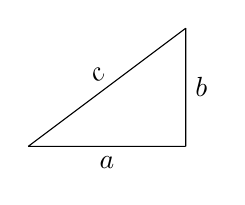
\begin{tikzpicture}[scale=0.5]
    \draw (3,0) -- node[sloped,above]{$c$} (7,3)
          (3,0) -- node[below]{$a$} (7,0)
          (7,0) -- node[right]{$b$} (7,3);
  \end{tikzpicture}
\end{center}
It lies at the heart of algebraic geometry,
relating the three side lengths of a right-angled triangle in an elegant way:

\medskip
\noindent{\bf Pythagoras' Theorem}
\[
  a^2 + b^2 = c^2
\]
There are several picture proofs of this theorem
but we will present just one, this time without any accompanying words.


\medskip
\noindent {\em Proof}

\begin{center}
  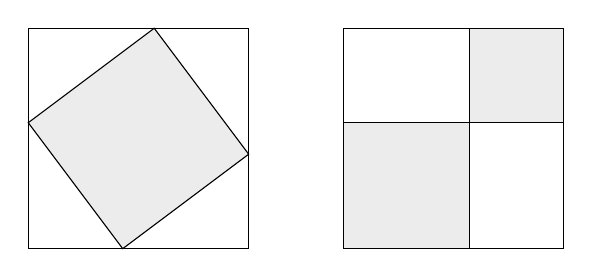
\begin{tikzpicture}[scale=0.4]
%    \draw [fill,pattern=crosshatch, pattern color=white!85!gray,draw=black] (0,0)--(0,7)--(7,7)--(7,0)--cycle;
    \draw [fill=white,draw=black] (0,0)--(0,7)--(7,7)--(7,0)--cycle;
    \draw [fill=white!85!gray,draw=black] (3,0)--(0,4)--(4,7)--(7,3)--cycle;
    \begin{scope}[xshift=10cm]
      \draw [fill,white!85!gray,draw=black] (0,0)--(4,0)--(4,4)--(0,4)--cycle;
      \draw [fill,white!85!gray,draw=black] (4,4)--(7,4)--(7,7)--(4,7)--cycle;
%      \draw [fill,pattern=crosshatch, pattern color=white!85!gray,draw=black]
      \draw [fill=white,draw=black]
      (4,0)--(4,4)--(7,4)--(7,0)--cycle;
%      \draw [fill,pattern=crosshatch, pattern color=white!85!gray,draw=black]
      \draw [fill=white,draw=black]
      (0,4)--(0,7)--(4,7)--(4,4)--cycle;
    \end{scope}
  \end{tikzpicture}
\end{center}
\hfill$\square$

\medskip
When you see the picture and convince yourself that it proves
Pythagoras' theorem, you are, again, telling a story
%constructing a narrative
that could also be useful (and amended as necessary) if you were to
describe the proof to a friend.

%\iffalse
%Can you see how the proof leads you to Pythagoras' Theorem?
%If you get stuck, then you can cheat (dishonourably) by looking at the footnote on
%this page.\footnote{\begin{tikzpicture}
%    \node[rotate=180] at (0  ,-0.5) {The area of this square is $(a+b)^2 = a^2 + b^2 + 2ab$
%                                     and is also $4(\frac{1}{2}ab) + c^2 = 2ab + c^2$.\\};
%    \node[rotate=180] at (0.6, 0  ) {Equating these two without the $2ab$ terms gives us
%                                     the identity $a^2 + b^2 = c^2$.};
%  \end{tikzpicture}}
%\fi

\medskip

\subsection*{Areas of triangles: Right for the wrong reasons}
\noindent
Just like written formal proofs,
picture proofs can contain flaws or holes
that are not always immediately obvious.
Let us for instance prove the following simple fact:

\begin{theorem}
\label{thm:triarea}
The area of a triangle is half of its base width times its height.
\end{theorem}

\noindent {\em Proof}

\begin{center}
  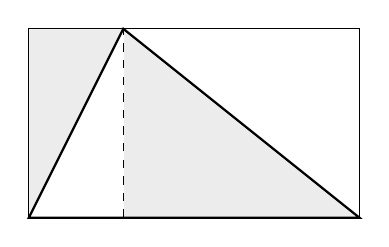
\begin{tikzpicture}[scale=0.6]
    \fill[fill=white!85!gray  ,draw=white] (0,0) -- (0,4) -- (2,4) -- cycle;
    \fill[fill=white!85!gray  ,draw=white] (2,0) -- (7,0) -- (2,4) -- cycle;
    \draw (0,0) rectangle (7,4);
    \draw[thick]  (0,0)--(2,4)--(7,0)--cycle;
    \draw[dashed] (2,0)--(2,4);
  \end{tikzpicture}
\end{center}
The big triangle is formed from two smaller triangles, one white and white grey,
each of which has an different-coloured twin outside the big triangle.
The area inside the big triangle is therefore the same as the area outside of it.
The four triangles form the full rectangle,
so the big triangle's area is half that of the rectangle
which is the base width times the height.
\hfill$\square$

\medskip
This is a simple proof of a simple theorem,
and you might even have understood it at a glance,
without even reading the explaining text.
However, the proof is wrong!
Or rather, the proof does not work for triangles having
an angle greater than $90^\circ$.

By using the picture below and by modifying our arguments from above,
can you fix the proof by showing that the theorem also holds for
triangles with an angle greater than~$90^\circ$?
({\em Hint}: First identify the rectangle that has twice the triangle's area.)
\begin{center}
  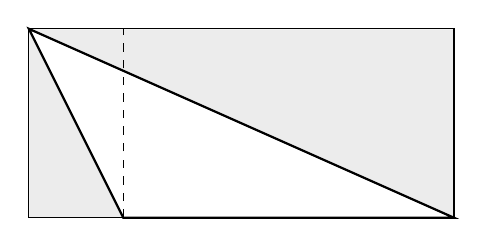
\begin{tikzpicture}[scale=0.6]
    \fill[fill=white!85!gray  ,draw=white] (-2,4) -- (0,0) -- (-2,0) -- cycle;
    \fill[fill=white!85!gray  ,draw=white] (-2,4) -- (7,4) -- ( 7,0) -- cycle;
    \draw[thick] (0,0) -- (-2,4) -- (7,0) -- cycle;
    \draw (-2,0) rectangle (7,4);
    \draw[dashed] (0,0) -- (0,4);
%    \fill[fill opacity=.2,blue] (-2,0)--(7,0)--(7,4)--(-2,4)--cycle;
%    \fill[pattern=crosshatch,pattern color=red] (-2,0)--(0,0)--(0,4)--(-2,4)--cycle;
  \end{tikzpicture}
\end{center}

\medskip

\subsection*{Explaining ideas}
\noindent
Ideally, a proof should not only convince us that some mathematical theorem is true;
it should also explain the theorem so that we understand it, not just believe it.
A picture proof is particularly useful if it can provide us with this insight
at a quick glance.
So far, our proofs have been nice and elegant
but they might not all have provided you with clear insight.
Let us therefore look at a picture proof that clearly explains as well as convinces.

\medskip

\subsection*{To infinity and beyond}
\noindent
%Stereographic project and equivalence of $\mathbb{R}$ and $(0,1)$}
Two finite sets have the same size if we can match each element of the one set
with an element of the other set, and vice versa. For instance,
the sets $\{1,2,4\}$ and $\{a,b,c\}$ have the same size (3)
since we can match up their elements, for instance in the obvious way:
\[
  1 \,\text{---}\, a \qquad
  2 \,\text{---}\, b \qquad
  4 \,\text{---}\, c
\]
If our sets are infinite, then we could use the same matching-up criterium
to determine whether the sets are, in this sense, of the same size.

\begin{theorem}
\label{thm:infbij1}
The real interval $(0,1)$ can be matched up with the whole set of real numbers~$\mathbb{R}$.
\end{theorem}

\noindent {\em Proof}

\begin{center}
  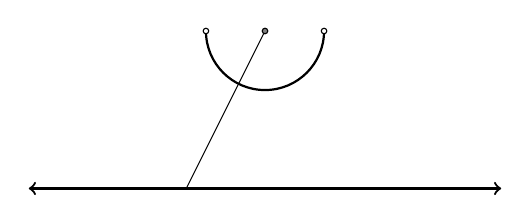
\begin{tikzpicture}[scale=0.5]
    \draw[<->,thick] (-6  ,-4) -- (6,-4);
    \draw[thick] (-1.5, 0) arc (180:360:1.5);
    \draw (0,0) -- (-2,-4);
    \foreach \x in {-1,1}{\fill[fill=white,draw=black] (1.5*\x,0) circle (2pt);};
    \fill[fill=gray,draw=black] (0,0) circle (2pt);
  \end{tikzpicture}
\end{center}
Here, the interval $(0,1)$ is drawn as a semicircle, and $\mathbb{R}$ as an infinite line.
Drawing a line starting from the semicircle's center, down through the $(0,1)$ interval,
and onto $\mathbb{R}$ gives a direct matching up of the two sets.
\hfill$\square$

\medskip

This idea of matching up can be further used to prove even more
interesting (and perhaps even counter-intuitive) results, such as that
there are ``equally many'' rational and natural numbers using a proof
famously known as the ``diagonal argument'':

\begin{theorem}
\label{thm:infbij2}
The natural numbers $\mathbb{N} = \{1,2,\ldots\}$ can be matched up with
all pairs $\mathbb{N}^2 = \{(1,1),(1,2),(2,1),\ldots\}$ of natural numbers.
\end{theorem}

\noindent {\em Proof}

\begin{center}
%  This commented solution requires fading subpackage which fucks things up for many pdf viewers
%
%    \path [scope fading=north, fading angle=-45] (-0.5,-0.5) rectangle (5.5,5.5);
%    \foreach \x in {1,...,5}{\draw (\x,0) -- (0,\x); \draw (5.5,5.5-\x) -- (5.5-\x,5.5);}
%    \draw (0,0) -- (1,0); \draw (2,0) -- (3,0); \draw (4,0) -- (5,0  );
%    \draw (0,1) -- (0,2); \draw (0,3) -- (0,4); \draw (0,5) -- (0,5.5);
%    \foreach \x in {0,...,5}{
%      \foreach \y in {0,...,5}{
%        \fill[fill=white,draw=transparent!100] (\x,\y) circle (3mm);}};
%
  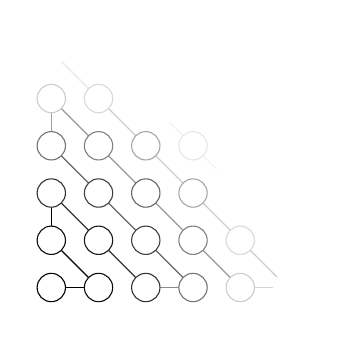
\begin{tikzpicture}[scale=0.6]
    \path (-0.5,-0.5) rectangle (5.5,5.5);
    \foreach \x in {1,...,5}{\pgfmathsetmacro\z{0.2*\x-0.2}\definecolor{mycolor}{rgb}{\z,\z,\z}
      \draw[mycolor] (\x,0) -- (0,\x);} %\draw[mycolor] (5.5,5.5-\x) -- (5.5-\x,5.5);}
      \draw (0,0) -- (1,0); \draw[white!10!gray] (2,0) -- (3,0); \draw[white!66!gray] (4,0) -- (5,0);
      \draw (0,1) -- (0,2); \draw[white!25!gray] (0,3) -- (0,4); \draw[white!90!gray] (1,4) -- (0,5); %\draw (0,5) -- (0,5.5);
      \draw[white!90!gray] (2.5,3.5) -- (3.5,2.5); %\draw (0,5) -- (0,5.5);
    \foreach \x in {0,...,5}{
      \foreach \y in {0,...,5}{\pgfmathsetmacro\z{0.05*\x*\x+0.05*\y*\y}
                \definecolor{mycolor}{rgb}{\z,\z,\z}
        \fill[fill=white,draw=mycolor] (\x,\y) circle (3mm);}};
  \end{tikzpicture}
\end{center}
Draw a line through the pairs in $\mathbb{N}^2$,
presented as the infinite array of circles above.
This matches up the numbers $\mathbb{N}$ and the pairs $\mathbb{N}^2$:
1 is matched up with $(1,1)$;
2 is matched up with $(2,1)$;
3 is matched up with $(1,2)$;
4 is matched up with $(1,3)$;
and so on.
\hfill$\square$

\medskip

\subsection*{But are these pictures really proofs?}
\noindent
We have presented a variety of our favourite picture proofs
and hope that you have enjoyed them too.\footnote{You can find many more nice picture proofs,
for instance in the books {\sl Proofs without Words} and {\sl Proofs without Words II} by Roger B.\ Nelsen.}
But, you might ask, are these {\em really} proofs?
Can they stand alone without accompanying text?
Are they too imprecise --- or are they sometimes too specific,
for instance to represent induction arguments or the infinite?
Do we really need pictures when words and symbols might suffice?
And do these pictures allow us to find new results,
or are they just pretty distractions?
These and other questions are sometimes asked by
some mathematicians, and the ensuing discussions for and against
picture proofs can quickly lead to very deep and interesting questions
about the nature of mathematics, the nature of truth,
the nature of the world, and the nature of our own understanding.

We will not even scratch the surface of these fascinating questions here in this article
but leave it up to you, the reader, to search for ways of answering them yourself.
In that process,
you may perhaps consider subquestions
%by introspection
such as:
Were you convinced by each of these proofs?
Would you prefer a formal written proof to any of these picture proofs?
Or, if you liked them and were convinced by them,
can you find more nice picture proofs of your own?

As a final challenge, and to show how these pictures can lead to new results,
we challenge you to prove that a pyramid with width, length, and height 1 has volume $\frac{1}{3}$,
by using Theorem~\ref{thm:square_sum} to fill in the details of the following picture proof:%
\footnote{This proof was first published (in written form) in 1086 AD by Shen Kuo,
  who wrote about {\em zao wei zhi shu}, or ``the art of piling up very small things".
  We here see an early instance of infinite limits and integration.
  (See [M.-K.~Sui, {\sl Pyramid, pile, and sum of squares},
   Historia Math.~{\bf 8} (1981), 61--66].)}

\newcommand{\pyramidv}[1]{
  \foreach \x in {#1,...,1} {
    \fill[fill=white!50!gray,draw=black] (0,-\x*3*\zc) -- ++(0,2*\zc) -- ++(-\x*\xc,\x*\zc) -- ++(0,-2*\zc) -- cycle;
    \fill[fill=white!75!gray,draw=black] (0,-\x*3*\zc) -- ++(0,2*\zc) -- ++( \x*\xc,\x*\zc) -- ++(0,-2*\zc) -- cycle;
    \fill[fill=white        ,draw=black] (0,-\x*3*\zc+2*\zc) -- ++(\x*\xc,\x*\zc) -- ++(-\x*\xc,\x*\zc) -- ++(-\x*\xc,-\x*\zc) -- cycle;}}

\begin{center}
  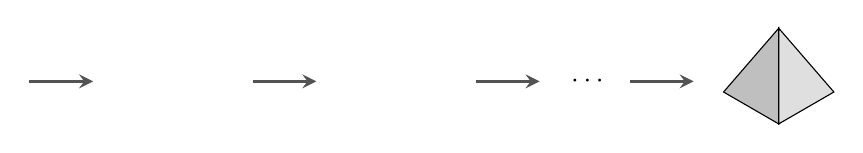
\begin{tikzpicture}[scale=.135,shift={(0,0)}]
    \foreach \xx in {3,4,5}{
      \begin{scope}[shift={(21*\xx-63,0)},scale=3/\xx]
        \pyramidv{\xx}
      \end{scope}
      \draw[draw=darkgray!90, fill=darkgray!90, very thick,>=stealth,->] (21*\xx-55.5,-5) -- ++(6,0);}
    \draw (60,-5) node{$\cdots$};
    \draw[draw=darkgray!90, fill=darkgray!90, very thick,>=stealth,->] (64,-5) -- ++(6,0);
    \begin{scope}[shift={(78,-9)}]
      \fill[fill=white!50!gray,draw=black] (0,0) -- (0,9*\zc) -- (-3*\xc,3*\zc) -- cycle;
      \fill[fill=white!75!gray,draw=black] (0,0) -- (0,9*\zc) -- ( 3*\xc,3*\zc) -- cycle;
    \end{scope}
  \end{tikzpicture}
\end{center}
